\documentclass[tikz,border=8pt]{standalone}
\usepackage{amsmath,amssymb}
\usetikzlibrary{arrows.meta,calc,decorations.pathreplacing,patterns,shapes.geometric,positioning,shadings}

\begin{document}
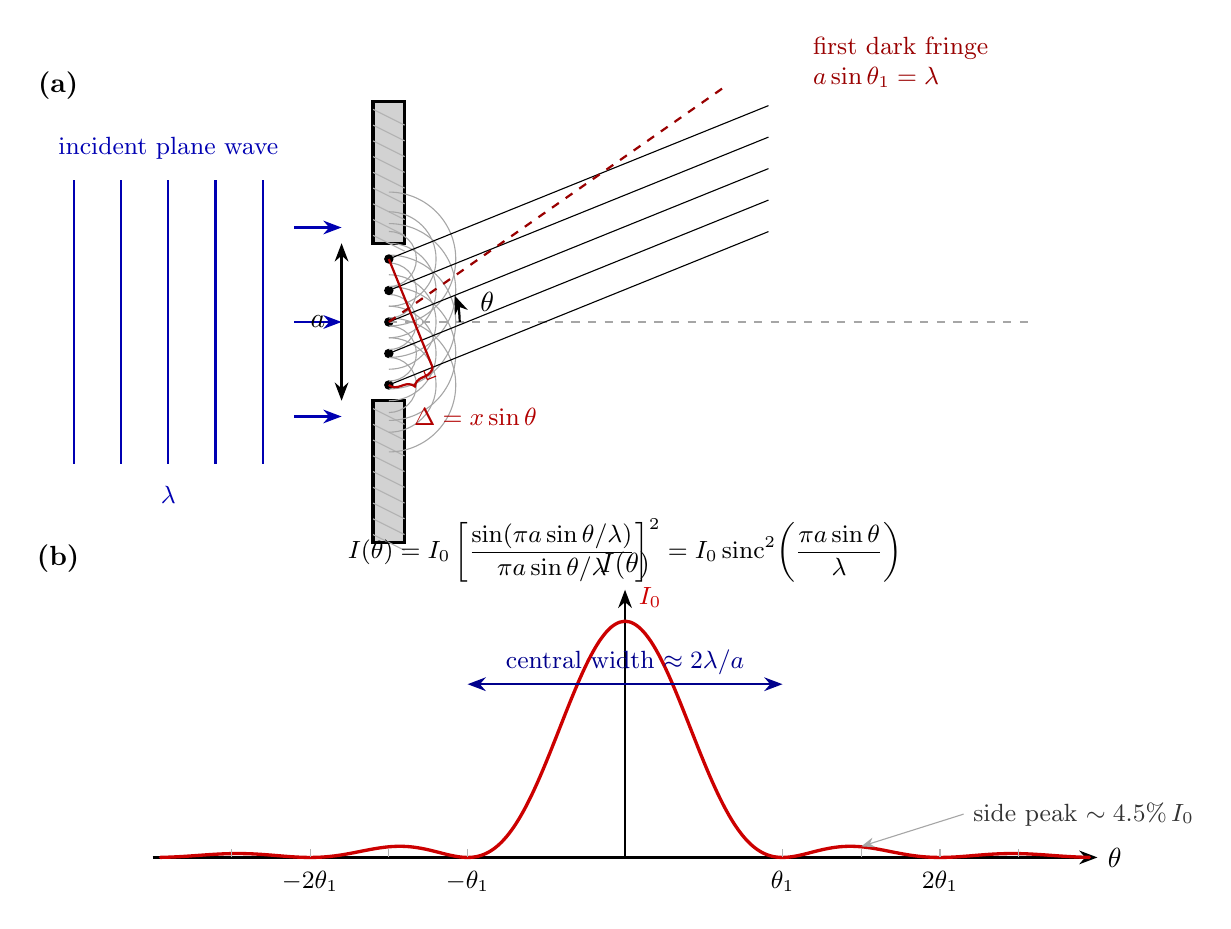
\begin{tikzpicture}[>=Stealth]

% =====================================================
% TOP PANEL: Geometry of single-slit diffraction
% =====================================================

% --- Incident plane wavefronts (left) ---
\foreach \xw in {-7.0,-6.4,-5.8,-5.2,-4.6} {
  \draw[blue!70!black,thick] (\xw,-1.8) -- (\xw,1.8);
}
% Arrows showing incident direction
\foreach \yarr in {-1.2,0,1.2} {
  \draw[blue!70!black,->,thick] (-4.2,\yarr) -- (-3.6,\yarr);
}
\node[blue!70!black] at (-5.8,2.2) {\small incident plane wave};
\node[blue!70!black] at (-5.8,-2.2) {\small $\lambda$};

% --- Opaque screen (barrier) with slit of width a ---
% a = 2 units in figure (from y=-1.0 to y=1.0). Center at origin.
\draw[line width=1.2pt,fill=gray!35] (-3.2,1.0) rectangle (-2.8,2.8);
\draw[line width=1.2pt,fill=gray!35] (-3.2,-2.8) rectangle (-2.8,-1.0);
% Hatch
\foreach \yh in {1.1,1.3,1.5,1.7,1.9,2.1,2.3,2.5,2.7} {
  \draw[gray!60] (-3.2,\yh) -- (-2.8,\yh-0.2);
}
\foreach \yh in {-2.7,-2.5,-2.3,-2.1,-1.9,-1.7,-1.5,-1.3,-1.1} {
  \draw[gray!60] (-3.2,\yh) -- (-2.8,\yh-0.2);
}

% Slit width indicator a
\draw[<->,thick] (-3.6,-1.0) -- (-3.6,1.0);
\node at (-3.9,0) {$a$};

% --- Huygens secondary wavelets: discrete sources in slit ---
% Sources at y = -0.8, -0.4, 0, 0.4, 0.8 (5 sources spanning the slit)
\foreach \ys in {-0.8,-0.4,0,0.4,0.8} {
  \fill[black] (-3.0,\ys) circle (0.06);
  % two concentric grey arcs (secondary spherical waves to the right)
  \draw[gray!70,thin] (-3.0,\ys) ++(-90:0.35) arc (-90:90:0.35);
  \draw[gray!70,thin] (-3.0,\ys) ++(-90:0.6) arc (-90:90:0.6);
  \draw[gray!70,thin] (-3.0,\ys) ++(-90:0.85) arc (-90:90:0.85);
}

% --- Reference horizontal axis from slit center to screen ---
\draw[dashed,gray!70] (-3.0,0) -- (5.2,0);

% --- Parallel rays toward observation direction at angle theta ---
% Angle theta ~ 22 degrees for clarity
\def\thetaDeg{22}
\foreach \ys in {-0.8,-0.4,0,0.4,0.8} {
  \draw[black,thin] (-3.0,\ys) -- ++({cos(\thetaDeg)*5.2},{sin(\thetaDeg)*5.2});
}

% --- Angle theta marker at slit center ---
\draw[->,thick] (-2.1,0) arc (0:\thetaDeg:0.9);
\node at (-1.75,0.25) {$\theta$};

% --- Path difference construction: perpendicular from top source to ray from bottom source ---
% Top source at (-3, 0.8), bottom source at (-3, -0.8). Ray from bottom goes at angle theta.
% Draw perpendicular from top source onto the ray from bottom source.
% Direction of ray: (cos theta, sin theta). Foot of perpendicular from top source to ray from bottom:
% bottom source B = (-3,-0.8); top source T = (-3,0.8). Vector BT = (0, 1.6).
% Projection onto direction d = (cos th, sin th): 1.6*sin(theta) = Delta
% Foot F = B + (BT.d)*d
\pgfmathsetmacro{\proj}{1.6*sin(\thetaDeg)}
\pgfmathsetmacro{\Fx}{-3.0 + \proj*cos(\thetaDeg)}
\pgfmathsetmacro{\Fy}{-0.8 + \proj*sin(\thetaDeg)}

% Perpendicular segment (short red brace-like line) from top source to foot
\draw[red!70!black,thick] (-3.0,0.8) -- (\Fx,\Fy);
% Small right-angle square at foot
\pgfmathsetmacro{\rax}{\Fx - 0.12*cos(\thetaDeg) + 0.12*sin(\thetaDeg)}
\pgfmathsetmacro{\ray}{\Fy - 0.12*sin(\thetaDeg) - 0.12*cos(\thetaDeg)}
\pgfmathsetmacro{\rbx}{\Fx - 0.12*cos(\thetaDeg)}
\pgfmathsetmacro{\rby}{\Fy - 0.12*sin(\thetaDeg)}
\pgfmathsetmacro{\rcx}{\Fx + 0.12*sin(\thetaDeg)}
\pgfmathsetmacro{\rcy}{\Fy - 0.12*cos(\thetaDeg)}
\draw[red!70!black,thin] (\rbx,\rby) -- (\rax,\ray) -- (\rcx,\rcy);

% Label Delta = x sin theta along the segment B to F (path difference for bottom source)
\draw[decorate,decoration={brace,amplitude=4pt,mirror},red!70!black,thick]
  (-3.0,-0.8) -- (\Fx,\Fy);
\node[red!70!black] at (-1.9,-1.2) {\small $\Delta = x\sin\theta$};

% --- First-order dark fringe direction dashed ---
% First dark fringe: sin theta_1 = lambda/a. Angle ~ illustrative; use different angle for visual.
\def\thetaOneDeg{35}
\draw[dashed,red!60!black,thick] (-3.0,0) -- ++({cos(\thetaOneDeg)*5.2},{sin(\thetaOneDeg)*5.2});
\node[red!60!black,align=left] at (3.5,3.3) {\small first dark fringe\\[-1pt] \small $a\sin\theta_1=\lambda$};

% =====================================================
% BOTTOM PANEL: Intensity I(theta) with sinc^2 profile
% =====================================================

% Shift coordinate: bottom panel y-offset
\begin{scope}[yshift=-6.8cm]

% Horizontal theta-axis
\draw[->,thick] (-6.0,0) -- (6.0,0) node[right] {$\theta$};
% Vertical intensity axis
\draw[->,thick] (0,0) -- (0,3.4) node[above] {$I(\theta)$};

% sinc^2 curve
% Use u = x, I = (sin(pi u)/(pi u))^2 scaled; but with x in units such that first zero at u=1
% We set visual scale: first zero at x = +/-2 in figure. So parameter u = x/2.
% I(x) = 3.0 * ( sin(pi*x/2) / (pi*x/2) )^2  [peak 3.0 at x=0]
% We'll plot with many samples.

\draw[red!80!black,very thick,line cap=round,samples=401,domain=-5.9:5.9,smooth]
  plot ({\x},{3.0*(sin(deg(pi*\x/2))/(pi*\x/2))^2});

% Mark zeros at x = +/-2, +/-4 etc with dashed verticals
\foreach \xz in {-5,-4,-3,-2,2,3,4,5} {
  \draw[dashed,gray!60] (\xz,0) -- (\xz,0.15);
}
% Label first zeros
\node[below] at (-2,-0.05) {\small $-\theta_1$};
\node[below] at (2,-0.05) {\small $\theta_1$};
\node[below] at (-4,-0.05) {\small $-2\theta_1$};
\node[below] at (4,-0.05) {\small $2\theta_1$};

% Central peak label
\node[red!80!black,above right] at (0.05,3.05) {\small $I_0$};
% Central width 2 lambda/a indicator (double arrow across first zeros)
\draw[<->,thick,blue!55!black] (-2,2.2) -- (2,2.2);
\node[blue!55!black,above] at (0,2.2) {\small central width $\approx 2\lambda/a$};

% Side peak markers: peak at x ~ 3 (3pi/2 in scaled variable maps to x=3), height ~ 0.045*3.0 = 0.135
\draw[<-,thin,gray!70] (3,0.14) -- (4.3,0.55);
\node[gray!40!black,right] at (4.3,0.55) {\small side peak $\sim 4.5\%\, I_0$};

% Formula label above bottom panel
\node at (0,3.9) {\small $I(\theta) = I_0\left[\dfrac{\sin(\pi a\sin\theta/\lambda)}{\pi a\sin\theta/\lambda}\right]^2 = I_0\,\mathrm{sinc}^2\!\left(\dfrac{\pi a\sin\theta}{\lambda}\right)$};

\end{scope}

% =====================================================
% Panel labels
% =====================================================
\node[font=\bfseries] at (-7.2,3.0) {(a)};
\node[font=\bfseries] at (-7.2,-3.0) {(b)};

\end{tikzpicture}
\end{document}
